\documentclass{beamer}

% balíčky

\usepackage[size=custom, width=120, height=120, scale=0.9, margin=0pt]{beamerposter}
\usepackage{../socstyle}
\usepackage[absolute,overlay]{textpos}

\usepackage[font={footnotesize}]{caption}
\usepackage[font={footnotesize}]{subcaption}

\usepackage{multicol}

\usepackage{parskip}
\renewcommand{\baselinestretch}{1.1}
\setlength{\parskip}{18pt} 
% \renewcommand{\arraystretch}{0.5}

\usepackage{tcolorbox}
\tcbuselibrary{breakable}
\definecolor{myblue}{HTML}{172983}
\tcbset{
		colback=myblue!5!white,
		colframe=myblue!75!black,
		fonttitle=\fontsize{48}{35}\selectfont\bfseries,
		boxrule=5pt,
		boxsep=18pt,
		parbox=false
}

\usepackage{asymptote}
\def\asydir{asy}

\usepackage[backend=biber, url=true, style=numeric, sorting=none]{biblatex}
\usepackage{url}
\addbibresource{/home/adam/tex/soc.bib}
\renewcommand*{\bibfont}{\footnotesize}

% délky
\newlength{\head}
\setlength{\head}{20cm}

\newlength{\sep}
\setlength{\sep}{1.5cm}

\newlength{\vyska}
\setlength{\vyska}{\paperheight}
\addtolength{\vyska}{-\head}

\newlength{\vyskaA}
\setlength{\vyskaA}{\vyska}
\addtolength{\vyskaA}{-2\sep}

\newlength{\vyskaB}
\setlength{\vyskaB}{\vyska}
\addtolength{\vyskaB}{-2\sep}

\newlength{\vyskaC}
\setlength{\vyskaC}{\vyska}
\addtolength{\vyskaC}{-2\sep}

\newlength{\side}
\setlength{\side}{30cm}
\addtolength{\side}{-2\sep}

\newlength{\main}
\setlength{\main}{60cm}
\addtolength{\main}{-2\sep}

\newlength{\newparskip}
\setlength{\newparskip}{12pt}

\setlength{\baselineskip}{82pt}

% témata
\usetheme{Rochester}
\usecolortheme{seahorse}

% posraný zarovnávání
\newlength{\headP}
\setlength{\headP}{\head}
\addtolength{\headP}{-\sep}
\setbeamertemplate{headline}{%
\leavevmode%
  \hbox{%
    \begin{beamercolorbox}[wd=\paperwidth,ht=\headP,dp=0pt]{bg=green}%
    \end{beamercolorbox}%
  }
}
\setbeamertemplate{footline}[frame number]{}
\setbeamertemplate{navigation symbols}{}
\setbeamertemplate{footline}{} 
\setbeamertemplate{bibliography item}{\insertbiblabel}

% asi naprd definice
\title{Mechanika rodin planetek \\ s aplikací na rodinu Eunomia}
\author{Adam Křivka \\ \and doc. Mgr. Miroslav Brož, Ph.\,D.}
\institute{Cyrilometodějské gymnázium a střední odborná škola pedagogická Brno,\\ Lerchova 63, 602 00 Brno}


% ----------


\begin{document}

\begin{frame}

\begin{columns}[t]

\begin{column}{\sep}
\end{column}
\begin{column}{\side}
	\begin{tcolorbox}[title=Planetky ve sluneční soustavě\phantom{Úy},height=0.335\vyskaA,parbox=false]
		\textbf{Planetky} jsou nejpočetnější a svým způsobem nejzajímavější skupinou těles ve~\textbf{sluneční soustavě}. První planetka byla objevena v roce 1801, v dnešní době je již známo přes půl milionu planetek.\\[\newparskip]

		V~\textbf{hlavním pásu planetek} mezi \textit{Marsem} a~\textit{Jupiterem} tvoří planetky \textbf{rodiny} --- skupiny vzniklé \textbf{rozpadem} stejného mateřského tělesa, způsobeným srážkou s~jiným tělesem. V~naší práci se soustředíme na početnou rodinu \textit{Eunomia}, nacházející se ve středním hlavním pásu.\\[\newparskip]

		Studiem kolizních rodin můžeme zjistit mnoho informací o~vzniku sluneční soustavy a~její \textbf{dynamické struktuře}~\cite{nesvorny15}, např. můžeme podpořit teorii o~\textbf{Velkém pozdním bombardování} (angl. \textit{Late Heavy Bombardment})~\cite{broz13}.%\\[\newparskip]

\vspace{3cm}

		\begin{figure}[!htb]
			\begin{subfigure}[t]{0.44\textwidth}
			\centering
			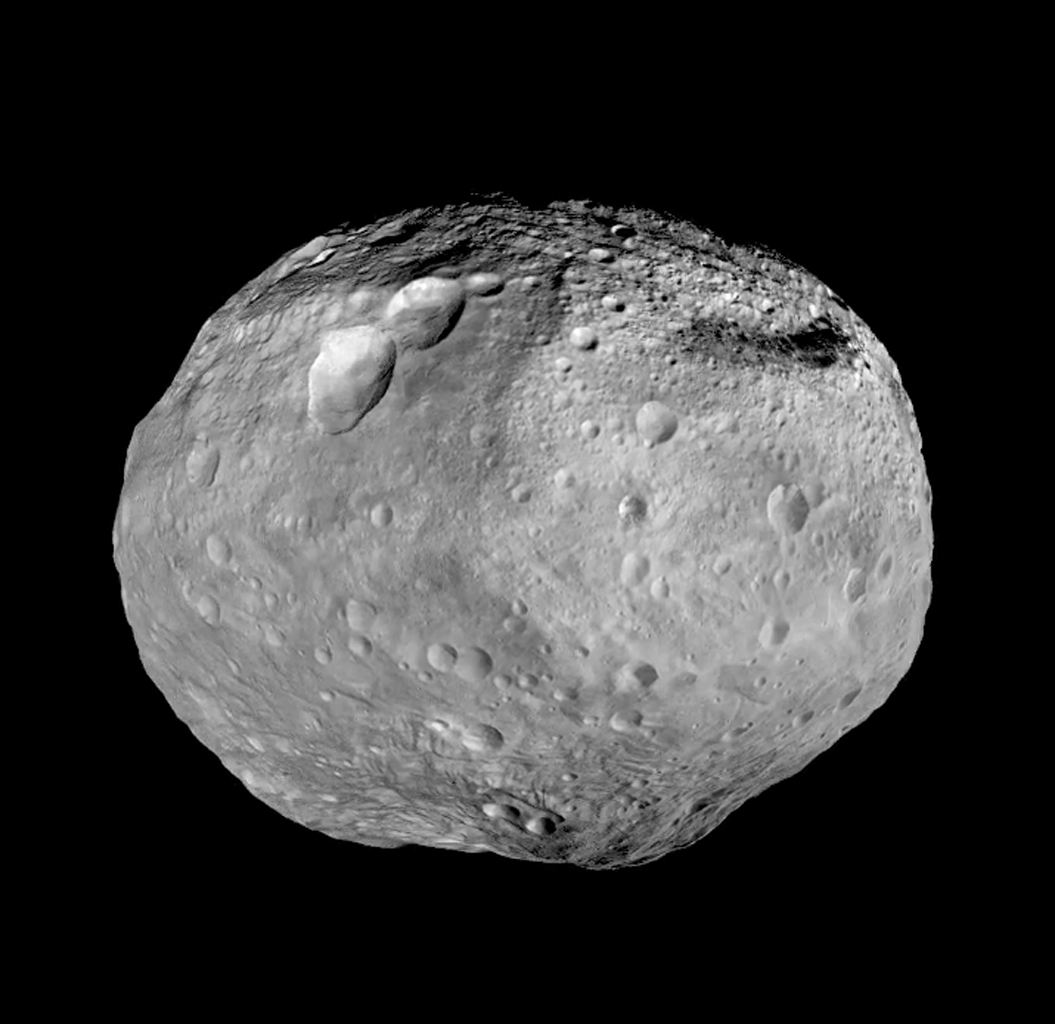
\includegraphics[width=0.95\textwidth]{../obr/vesta.jpg}
			\caption{Planetka \textit{(4) Vesta} --- druhé největší a~nejhmotnější těleso hlavního pásu planetek.} 
			\label{fig:vesta}
			\end{subfigure}
			\begin{subfigure}[t]{0.55\textwidth}
			\centering
			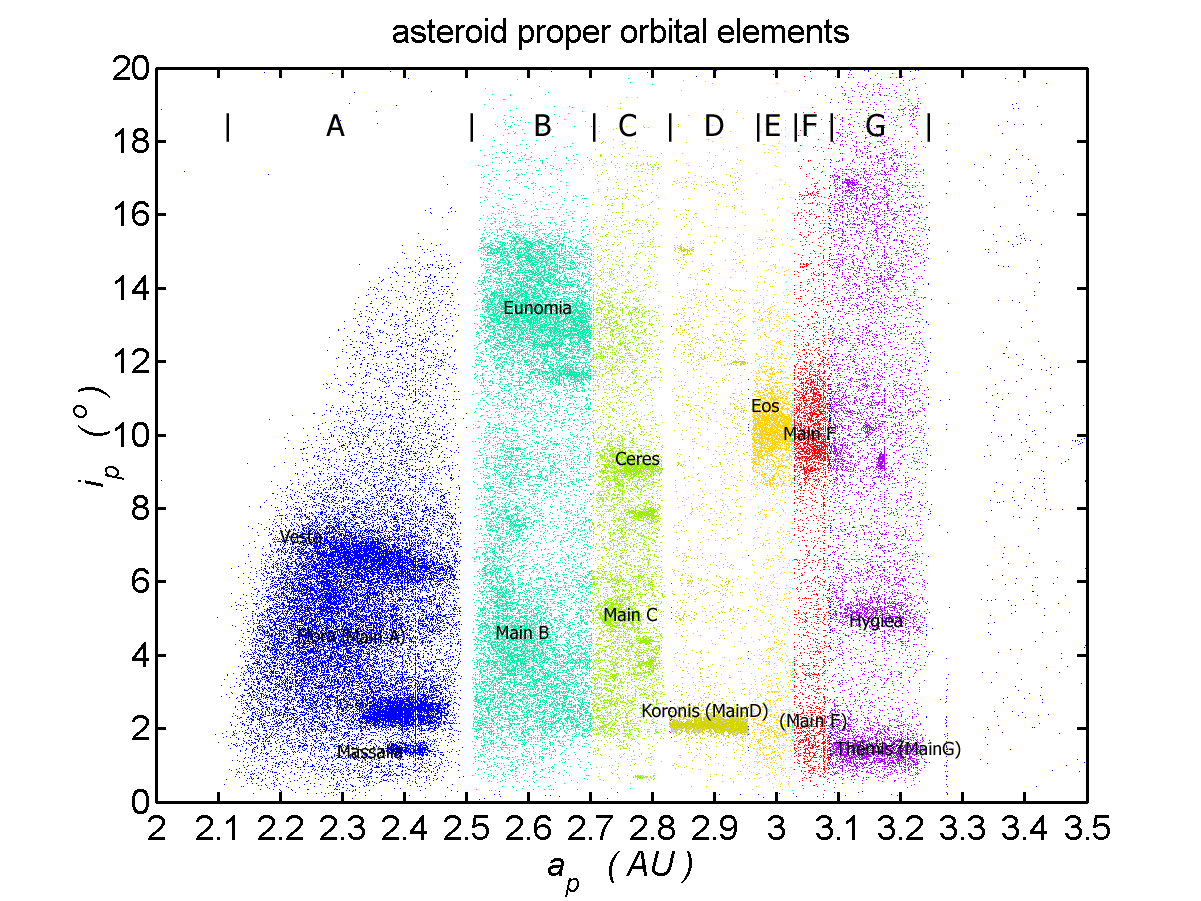
\includegraphics[width=1.0\textwidth]{../obr/mainbelt.png}
			\caption{Hlavní pás planetek v prostoru \textbf{vlastních elementů dráhy} --- vlastní hlavní poloosy $a_{\rm p}$ vlastní sklon $\sin I_{\rm p}$.} \label{fig:belt}
			\end{subfigure}
		\end{figure}
	\end{tcolorbox}

\vspace{\sep}

	\begin{tcolorbox}[title=Metody nebeské mechaniky\phantom{Úy},height=0.665\vyskaA]

		Základním problémem nebeské mechaniky je \textbf{problém $N$ těles}, podle \textbf{Newtonova gravitačního zákona}

		{\footnotesize
		\begin{align*} 
			\vec{F}_i = m_i\vec{a}_i &= -\sum_{\substack{j=1 \\ j\neq i}}^N G\frac{m_im_j}{\abs{\vec{r}_i-\vec{r}_j}^3}(\vec{r_i}-\vec{r_j})\,, \qquad{\rm pro}\ i\in\{1,\,2,\,\dots,\,N\}
		\end{align*}}

K simulaci orbitálního vývoje využíváme \textbf{numerického integrátoru SWIFT}, který počítá s 

	% \itemsep0em
\begin{itemize}
	\item \textbf{Jarkovského jevem},
	\item \textbf{YORP efektem},
	\item \textbf{náhodnými srážkami},
	\item \textbf{chaotickou difuzí}.  
\end{itemize}

		\begin{figure}[!htb]
			\centering 
			\begin{subfigure}[b]{0.45\textwidth}
			\centering 
			\asyinclude[width=1.0\textwidth]{../asy/f_euler.asy}
			\end{subfigure}
			\begin{subfigure}[b]{0.45\textwidth}
			\centering 
			\asyinclude[width=1.0\textwidth]{../asy/b_euler.asy}
			\end{subfigure}
			\caption{Ilustrace jednodušší integrační metody --- \textbf{Eulerovy metody} --- která je pricipielně té naší podobná.}
			% \caption{Ilustrace dopředné Eulerovy integrační metody pro dvě tělesa. Jsou ukázány první tři iterace. Šedá křivka znázorňuje analytické řešení problému dvou těles.} \label{fig:euler}
		\end{figure}
		% \vspace{-36pt}
		Oběžnou dráhu planetky kolem Slunce popisujeme \textbf{elementy dráhy}:
		\begin{itemize}
			% \itemsep0em
			\item \textbf{hlavní poloosa} $a$
			\item \textbf{excentricita} $e$
			\item \textbf{sklon} $I$ (nebo také $\sin I$) 
		\end{itemize}

\vspace{1cm}

Ty se v průběhu času mění působením \textbf{perturbací} (např. gravitační působení ostatních planet), můžeme je tedy přes dlouhé úseky \uv{průměrovat} na \textbf{střední} a na \textbf{vlastní elementy dráhy}.

		\vspace{1.0cm}

		\begin{figure}
			\centering
			\begin{subfigure}[b]{0.49\textwidth}
			\centering
			\includegraphics[width=1.0\textwidth]{../obr/atOF}
			\end{subfigure}
			\begin{subfigure}[b]{0.49\textwidth}
			\centering
			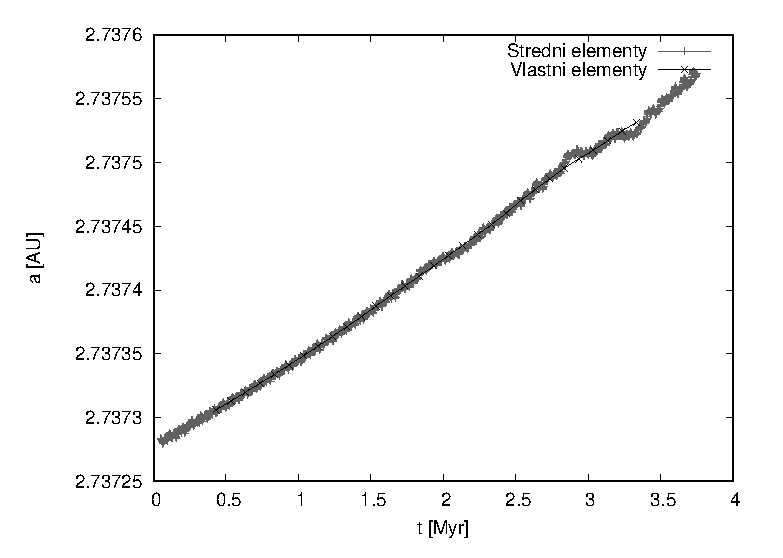
\includegraphics[width=1.0\textwidth]{../obr/atFP}
			\end{subfigure}
			\caption{\ Porovnání \textbf{oskulační} (aktuální) a \textbf{střední} hlavní poloosy (vlevo) a \textbf{střední} a~\textbf{vlastní} hlavní poloosy (vpravo) pro simulaci jedné planetky po dobu $3,76$ miliónů let.}
		\end{figure}
		% \vspace{-48pt}
		\begin{tabularx}{\textwidth}{p{12cm}X}

		\

		K určení členů rodiny používáme \textbf{hierarchickou shlukovací metodu} (HCM) --- v prostoru $(a_{\rm p},\,e_{\rm p},\sin I_{\rm p})$ si zvolíme hraniční vzájemnou \uv{vzdálenost} těles $v_{\rm cutoff}$ (s jednotkami rychlosti), podle které pak určíme členy (začneme u mateřského tělesa \textit{(15) Eunomia}).

		&
		\begin{figure}
			\centering
			\includegraphics[width=0.4\textwidth]{../obr/Nv_edit.png}
			\caption{Závislost počtu členů rodiny \textit{Eunomia} na zvolené hraniční rychlosti $v_{\rm cutoff}$ při použití metody HCM.}
			% Počet členů prudce vzroste při přechodu z~$43$ na $44\,{\rm m/s}$, což je způsobené velkou vzdáleností prvního nejbližšího tělesa od mateřského \textit{(15) Eunomia}. Dále vzroste prudce při přechodu z~$46$ na $47\,{\rm m/s}$, což je způsobené splynutím s~rodinou Adeona.
		\end{figure}
		\end{tabularx}
		\vspace{-0.5cm}
		{\begin{align*}
			v_{\rm cuttoff}=na_{\rm p}\sqrt{C_a\left(\frac{\Delta a_{\rm p}}{a_{\rm p}}\right)^2+C_e(\Delta e_{\rm p})^2+C_i(\Delta \sin i_{\rm p})^2}
		\end{align*}}

	\end{tcolorbox}

\vspace{\sep}

\end{column}

\begin{column}{2\sep}
\end{column}

\begin{column}{\main}
\begin{tcolorbox}[title=Určení členů rodiny Eunomia\phantom{Úy},height=0.25\vyskaB]

	K určení rodiny \textit{Eunomia} jsme použili metodu HCM. Dále jsme odstranili \textbf{přimísená tělesa} pomocí závislosti unášení ve \textbf{vlastní hlavní poloose} $\Delta a_{\rm p}$ na \textbf{absolutní hvězdné velikosti} $H$ a pomocí dvou spektroskopických metod --- závislosti \textbf{albed} $p_{\rm V}$ a $p_{\rm IR}$ a závislosti \textbf{barevných indexů} $a^*$ a $i-z$. Před odstraněním činil počet planetek 6503, po použití všech metod~6184.

	\vspace{-1.7cm}

	\begin{figure}[htbp]
		\begin{subfigure}[b]{0.3\textwidth}
			\centering
			\captionsetup{width=.88\linewidth}
			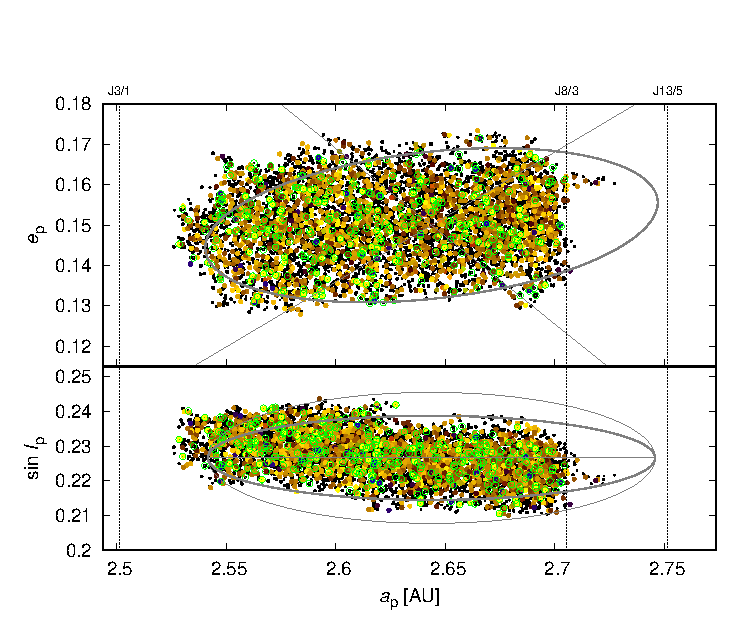
\includegraphics[width=1.0\textwidth]{../obr/ae_ai_wise}
			\caption{Pozorovaná rodina \textit{Eunomia} určená HCM s hodnotou $v_{\rm cutoff} = 44\,{\rm m/s}$ v~rovině \textbf{vlastní hlavní poloosy} $a_{\rm p}$ a~\textbf{vlastní excentricity} $e_{\rm p}$ (nahoře) a~v~rovině \textbf{vlastní hlavní poloosy} $a_{\rm p}$ a~\textbf{vlastního sklonu} $\sin I_{\rm p}$ (dole). Barevná škála odpovídá \textbf{albedu} $p_{\rm V}$ a~$p_{\rm IR}$ z~katalogu WISE \cite{nugent15}.}
% Nápisy J3/1, J8/3 a~J13/5 označují polohu \textbf{rezonancí středního pohybu} s~\textit{Jupiterem}. Šedé elipsy a~úsečky (degenerované elipsy) naznačují předpokládaný tvar rodiny, při rozpadu v bodě oběžné dráhy s hodnotami \textbf{pravé anomálie} $f=0^\circ,\,90^\circ,\,180^\circ$ (nahoře) a~jejího součtu s \textbf{argumentem pericentra} $\omega+f=0^\circ,\, 50^\circ,\, 90^\circ$ (dole), kde elipsou zvolenou pro další výpočety je elipsa pro hodnoty $f=90^\circ$ a~$\omega+f=50^\circ$.
			\label{fig:ae_ai_wise}
		\end{subfigure}
		\begin{subfigure}[b]{0.26\textwidth}
			\centering
			\captionsetup{width=.88\linewidth}
			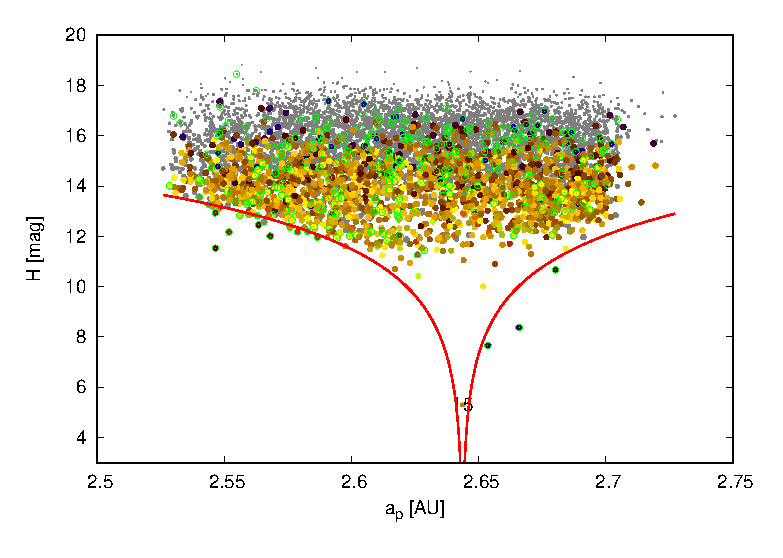
\includegraphics[width=1.0\textwidth]{../obr/aH_wise}
			\caption{Závislost unášení ve \textbf{vlastní hlavní poloose} $a_{\rm p}$ na~\textbf{absolutní hvězdné velikosti} $H$. Lze pozorovat typický tvar \uv{V}, který je způsoben počátečním \textbf{rychlostním polem} a~\textbf{Jarkovského jevem}, jenž je ještě zesílen vlivem \textbf{YORPu}, což způsobuje zvýšenou koncentraci malých planetek při okrajích rodiny.\newline\newline}
		\end{subfigure}
		\begin{subfigure}[b]{0.2\textwidth}
			\centering
			\captionsetup{width=.88\linewidth}
			\includegraphics[width=1.0\textwidth]{../obr/pV_pIR-crop}
			\caption{\textbf{Albeda} $p_{\rm V}$ (ve viditelném spektru) a~$p_{\rm IR}$ (v~infračerveném) z~katalogu WISE. Barvy neodpovídají reálnému zbarvení. Pro vyřazení \textbf{přimísených těles} touto metodou byly zvoleny hraniční hodnoty $0,05 \leq p_{\rm V} \leq 0,4$.\newline}
		\end{subfigure}
		\begin{subfigure}[b]{0.2\textwidth}
			\centering
			\captionsetup{width=.88\linewidth}
			\includegraphics[width=1.0\textwidth]{../obr/astar_iz-crop}
			\caption{\textbf{Barevné indexy} $a^*$ a~$i-z$ z~katalogu Sloan \cite{ivezic01}. Barvy neodpovídají reálnému zbarvení. Pro vyřazení \textbf{přimísených těles} byly zvoleny hraniční hodnoty $0\leq a^* \leq 0,3$ a~$-0,3\leq i-z \leq 0,3$.\newline\newline}
		\end{subfigure}
	\end{figure}

\end{tcolorbox}

\vspace{\sep}

\begin{tcolorbox}[title=Simulace orbitálního vývoje\phantom{Úy},height=0.75\vyskaB]
	\begin{tabularx}{\textwidth}{Xp{0.25\textwidth}}

	Při vytváření \textbf{syntetické} populace planetek jsme částicím přiřadili 
	\begin{itemize}
	% \itemsep0em
	\item \textbf{průměry} (dle pozorovaných dat --- zohlednili jsme \textbf{rozdělení velikostí}), 
	\item \textbf{albeda} (dle pozorovaných dat),
	\item \textbf{orientace rotačních os} (náhodně; vliv na \textbf{Jarkovského jev}),
	\item \textbf{úvodní rychlosti} (jako při \textbf{izotropním rozpadu} v bodě oběžné dráhy s hodnotami $f=90^\circ$ a $\omega+f=50^\circ$).
	\end{itemize}
	% . U průměrů jsme zohlednili \textbf{rozdělení velikostí} a při zpracovávání simulace jsme rozdělení korigovali tak, aby odpovídalo pozorovanému.

\

	Po dobu \textbf{$1,3$ miliardy let} jsme simulovali populaci \textbf{6210 částic}. Simulace byla spuštěna na \textbf{výpočetním clusteru Astronomického ústavu Univerzity Karlovy} a celkově se spotřebovalo přibližně \textbf{50000 CPU hodin} a celkový objem \textbf{binárních dat} je roven $164\,{\rm GB}$.

		&

		\vspace{-1cm}
		\begin{figure}
			\centering
			\captionsetup{width=0.2\textwidth}
			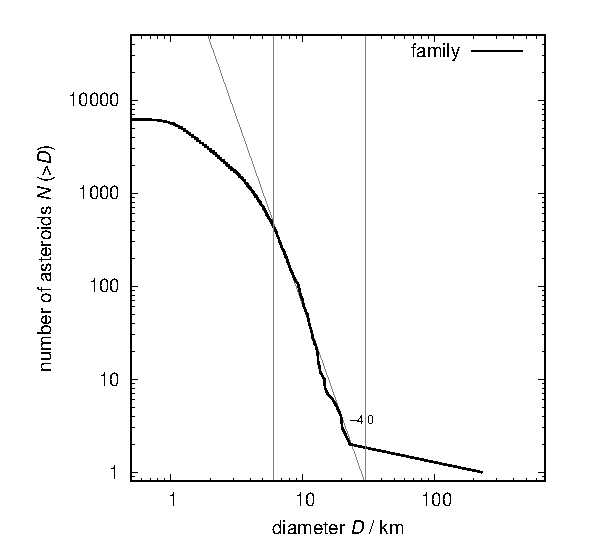
\includegraphics[width=0.2\textwidth]{../obr/size_distribution}
			\caption{\textbf{Histogram} četnosti velikostí planetek rodiny \textit{Eunomia}.} 
		% kde veličina $N({>}D)$ označuje počet planetek s~\textbf{průměrem} větším než $D$.
		%Jedná se o~\textbf{logaritmický graf} $(\log D,\,\log N({>}D))$, na kterém lze vztah mezi danými veličinami aproximovat přímkou, což znamená, že vztah mezi veličinami $D$ a~$N({>}D)$ je \textbf{mocninný}.}

		% Vodorovná část zcela vlevo je způsobena observační nedostatečností. Změna sklonu přímky prvního intervalu $D$ (vlevo, $q=-4$) na druhý interval $D$ (vpravo, $q=-1,2$) je důsledkem jednak prvotního rozpadu a~jednak druhotného vývoje --- tělesa se nadále srážejí, vytvářejí menší tělesa, která snáze opouštějí rodinu.
			\label{fig:sfd}
		\end{figure}
	\end{tabularx}

	\begin{figure}[t]
		\centering
		\includegraphics[width=0.24\textwidth]{../obr/ae_5.png}
		\includegraphics[width=0.24\textwidth]{../obr/ae_205.png}
		\includegraphics[width=0.24\textwidth]{../obr/ae_605.png}
		\includegraphics[width=0.24\textwidth]{../obr/ae_1105.png}
\\
		\includegraphics[width=0.24\textwidth]{../obr/ai_5.png}
		\includegraphics[width=0.24\textwidth]{../obr/ai_205.png}
		\includegraphics[width=0.24\textwidth]{../obr/ai_605.png}
		\includegraphics[width=0.24\textwidth]{../obr/ai_1105.png}
\\
		\includegraphics[width=0.24\textwidth]{../obr/ei_5.png}
		\includegraphics[width=0.24\textwidth]{../obr/ei_205.png}
		\includegraphics[width=0.24\textwidth]{../obr/ei_605.png}
		\includegraphics[width=0.24\textwidth]{../obr/ei_1105.png}
			\captionsetup{width=.88\linewidth}
			\caption{Výsledky simulace v~prostorech $(a_{\rm p},\,e_{\rm p})$, $(a_{\rm p},\,\sin I_{\rm p})$ a  $(e_{\rm p},\,\sin I_{\rm p})$ v~časech postupně $t=5,\,205,\,605,\,1105$ miliónů let. Nápisy J3/1, J8/3, J13/5 a~J5/2 označují nejvýznamnější \textbf{rezonance} s~\textit{Jupiterem}. Černá křivka nahoře označuje hranici oblasti, kde je hlavní poloosa a~excentricita tělesa taková, že dráha kříží dráhu \textit{Marsu}. Podobná hranice existuje i~pro \textbf{Jupiter}, ale ta se nachází mimo tyto grafy (přibližně kolem $e=0,65$). Fialový obdélník označuje oblast vybranou pro vzorek populace \textbf{pozadí}.} \label{fig:ae_sim}
	\end{figure}

\begin{multicols}{2}

\begin{itemize}
\item 
Kvůli specifickému výpočtu \textbf{vlastních elementů dráhy} z~počátečních rychlostí můžeme v~čase 5 miliónů let pozorovat mírně nesymetrický tvar simulované~rodiny. 

\item Mechanismus, kterým planetky \textbf{opouštějí} rodinu je následovný: působením \textbf{Jarkovského jevu} se planetka dostane do blízkosti nějaké \textbf{rezonance}, excentricita její oběžné dráhy se \textbf{zvýší} až začne \textbf{křížit dráhu} \textit{Marsu} nebo \textit{Jupiteru}, načež se pak při \textbf{blízkém přiblížení} prudce vychýlí ze své dráhy.

\vspace{2cm}
	\begin{figure}
		\centering
		\includegraphics[width=0.25\textwidth]{../obr/ae_obs.png}
		\caption{Graf $(a_{\rm p}, e_{\rm p})$ pro pozorovanou rodinu \textit{Eunomia}. Barevná škála označuje počet těles v~daném \textbf{boxu}.}
% Vpravo v oblasti $a_{\rm p}\in(2,7\,{\rm AU};\,2,75\,{\rm AU}),\ e_{\rm p}\in(0,16;\,0,18)$ lze pozorovat velmi malou rodinu příslušnou planetce $(53546)\ 2000\,BY6$, se kterou jsme v~naší simulaci, stejně jako s~ostatními rodinami, nepočítali.
	\end{figure}
\vfill\null\columnbreak

\item 
Tělesa nacházející se na počátku v blízkosti rezonance J5/2 byla velmi rychle rozptýlena, a tak se už na grafu pro $t=5$ miliónů let vůbec nevyskytují.

\item
\textbf{Rezonance} J8/3 a~J13/5 jasně rozdělují rodinu na tři části, které různě široké, a tudíž se v nich planetky rozptylují jinak.

\item 
Potvrzuje se, že \textbf{rezonance} J8/3 je silnější než \textbf{rezonance} J13/5 (planetky v~blízkosti rezonance J8/3 se v~čase 205 miliónů let rozšířily do pásu o~velikosti $0,05<e_{\rm p}<0,5$, zatímco v~blízkosti \textbf{rezonance} J13/5 pouze do pásu o~velikosti $0,1<e_{\rm p}<0,23$)

\item
Na grafu $(a_{\rm p},\,\sin I_{\rm p})$ můžeme pozorovat mírné \uv{\textbf{naklonění}} pozorované rodiny (část pod $a\approx2,62\,{\rm AU}$ má vyšší sklon $I_{\rm p}$), čehož si na rodině simulované bohužel zatím všimnout nemůžeme.

\item Postupem času koncentrace planetek v prostoru klesá, což je způsobeno \textbf{všemi} přítomnými \textbf{rezonancemi}.

% Lze vidět vliv \textbf{rezonancí středního pohybu} J3/1, J5/2, J8/3 a J13/5 --- v jejich blízkosti se \textbf{excentricity} planetek začnou zvyšovat, až se dostanou do oblasti, kde kříží dráhy \textit{Marsu} nebo \textit{Jupitera}, což znamená, že se planetka dříve nebo později některé z~těchto planet přiblíží a~její \textbf{hlavní poloosa} se náhle změní. Na prvním obrázku jsou data již zprůměrována z~prvních $10$ miliónů let, takže můžeme vidět, že se planetky, které se zřejmě na počátku nacházely v~blízkosti \textbf{rezonancí} J3/1, J8/3 a~J13/5, stihly rozptýlit a~narušily tak jinak zatím pravidelný tvar rodiny. 

\end{itemize}
\end{multicols}

\vspace{-1cm}

	\begin{figure}
		\centering
		\includegraphics[width=0.24\textwidth]{../obr/ae_scl_0006.png}
		\includegraphics[width=0.24\textwidth]{../obr/ae_scl_0206.png}
		\includegraphics[width=0.24\textwidth]{../obr/ae_scl_0606.png}
		\includegraphics[width=0.24\textwidth]{../obr/ae_scl_1106.png}
		\captionsetup{width=.88\linewidth}
		\caption{Graf $(a_{\rm p},\,e_{\rm p})$ simulované rodiny Eunomia pro $t=5,\ 205,\ 605, 1105$ miliónů let. Pozor na změnu barevné škály.} 

		\label{fig:ae_chi2}
	\end{figure}

\vspace{1.5cm}

\end{tcolorbox}
\vspace{\sep}
\end{column}

\begin{column}{2\sep}
\end{column}

\begin{column}{\side}
\begin{tcolorbox}[title=Stáří rodiny Eunomia\phantom{Úy},height=0.75\vyskaC]
{\centering \large \bfseries Metoda blackbox} \cite{broz19} \\[6pt]

{\small Planetky jak pozorované, tak simulované rodiny rozdělíme do \uv{boxů} v~prostoru $(a_{\rm p},\,e_{\rm p},\,\sin I_{\rm p})$ a~následně porovnáváme počty planetek v~jednotlivých \textbf{boxech}. Simulovanou populaci ještě \uv{smícháváme} se vzorkem \textbf{pozadí}, přičemž dodržujeme \textbf{rozdělení velikostí}. 

Na tento jednoduchý princip pak používáme statistickou metodu rozdělení \textbf{chí kvadrátu} ($\chi^2$) --- pro každý \textbf{box} vypočteme jeho příspěvek k~$\chi^2$ jako
\begin{align*}
	\frac{(N_{\rm sim}-N_{\rm obs})^2}{N_{\rm sim}+N_{\rm obs}}\,.
\end{align*}
}

% kde $N_{\rm sim}$, resp.\ $N_{\rm obs}$ označuje počet simulovaných, resp. pozorovaných těles v~daném \textbf{boxu}. Výslednou hodnotu $\chi^2$ potom dostaneme prostým sečtením všech příspěvků.\begin{figure}
	\begin{figure}
	\centering
	\includegraphics[width=0.49\textwidth]{../obr/ae_chi_0006.png}
	\includegraphics[width=0.49\textwidth]{../obr/ae_chi_0206.png}\\
	\includegraphics[width=0.49\textwidth]{../obr/ae_chi_0606.png}
	\includegraphics[width=0.49\textwidth]{../obr/ae_chi_1106.png}
	\captionsetup{width=.8\linewidth}
	\caption{Hodnota \textbf{chí kvadrátu} $\chi^2$ pro každý \textbf{box} v~prostoru $(a_{\rm p},\,e_{\rm p})$ pro $t=5,\ 205,\ 605,\ 1105$ miliónů let. Tečky označují \textbf{syntetickou} populaci i~s~přidaným \textbf{pozadím}.} 
	\label{fig:ae_chi2}
	\end{figure}

Můžeme vidět, že ze začátku se nejvíce odlišuje jádro rodiny kolem $2,65\,{\rm AU}$ (moc \textbf{syntetických} částic).\\[\newparskip]   

Kvůli silné \textbf{kontaminaci} rodinou \textit{Adeona} v oblasti $0,16<e<0.18$ jsme byli nuceni pozorované členy této rodiny ručně odstranit.\\[\newparskip]

Podařilo se nám pochopit \textbf{struktur}, které lze na našich grafech v prostorech $(a_{\rm p},\,e_{\rm p})$, $(a_{\rm p},\,\sin I_{\rm p})$ a  $(e_{\rm p},\,\sin I_{\rm p})$. Některé jevy (např. přílišná kompaktnost jádra) bohužel musíme připsat \textbf{nedostatečně dlouhému časovému úseku}, po který jsme rodinu \textit{Eunomia} simulovali. S velkou pravděpodobnstí můžeme říct, že rodina \textit{Eunomia} \textbf{není mladší} než $500$ miliónů let, ale zatím nedokážeme odhadnout (z důvodu ploché závislosti \textbf{chí kvadrátu} na čase), jaký je horní limit stáří rodiny Eunomia.\\[\newparskip]

\vspace{0.5cm}

	\begin{figure}
		\centering
		\includegraphics[width=0.7\textwidth]{../obr/chi2.eps}
		\captionsetup{width=0.8\linewidth}
		\caption{Závislost \textbf{redukovaného chí kvadrátu} na čase. Skok v čase přibližně \textbf{1125~miliónů let} je způsoben \textbf{úbytkem těles} v simulaci.}
	\end{figure}

\vspace{0.5cm}

	V~budoucnu plánujeme simulovat rodinu \textit{Eunomia} po \textbf{delší dobu} (4 miliardy let). Pravděpodobně dostaneme nějakou minimální (statisticky významnou) hodnotu \textbf{chí kvadrátu}, čímž budeme schopni přesně určit horní mez pro \textbf{stáří} rodiny \textit{Eunomia}.\\[\newparskip]   

	Další možností vylepšení je analýza \textbf{okolních rodin}, zejména rodiny \textit{Adeona}. %Přesné určení počtu jejích členů a~stáří by nám pomohlo v~analýze rodiny \textit{Eunomia}, mohli bychom např. v~momentu rozpadu rodiny \textit{Adeona} její částice do simulace přidat.
	Můžeme se také zaměřit jen na některé \textbf{taxonomické typy} planetek (rodina \textit{Eunomia} je \textbf{typu S}) nebo vyzkoušet \textbf{anizotropní rychlostní pole} --- simulovat různé typy rozpadu (\textbf{kráterování}, \textbf{reakumulace}, \textbf{katastrofický rozpad}). Dále můžeme vyzkoušet \textbf{různé vzorky pozadí} pro různé oblasti (mezi rezonancemi J8/3 a J13/5 je menší koncentrace pozorovaných těles než mezi rezonancemi J3/1 a J8/3).\\[\newparskip]

	Po \textbf{dokončení dlouhodobé simulace} plánujeme \textbf{publikaci} výsledků v~odborném časopisu (\textit{Icarus}).

\end{tcolorbox}
\vspace{\sep}
\begin{tcolorbox}[title=Reference\phantom{Úy},height=0.25\vyskaC]
	\printbibliography

	\tcblower

	\newrefsection{}
	\setbeamertemplate{bibliography item}[book]
	\nocite{fmt}
	\nocite{murray00}
	\nocite{brozphd}
	\printbibliography
\end{tcolorbox}
\end{column}

\begin{column}{\sep}
\end{column}

\end{columns}

\end{frame}

\end{document}
